\documentclass[12pt]{article}

\usepackage{tikz}

\begin{document}
	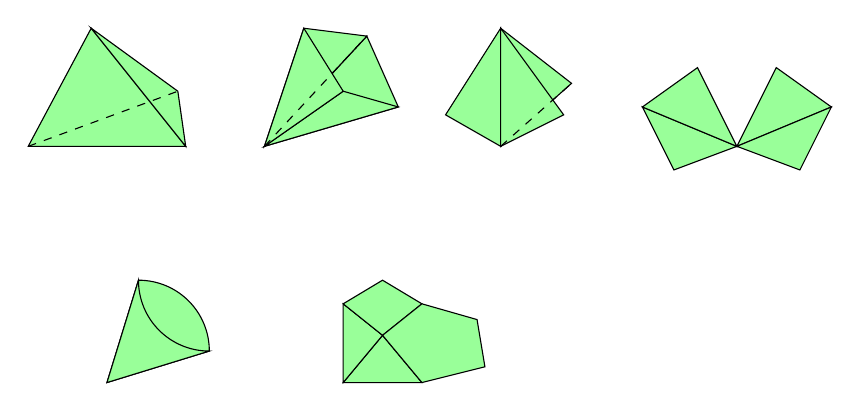
\begin{tikzpicture}
		% We need to define the drawing style
		[edges/.style={black, dashed},
		faces/.style={fill=green!40!white, draw=black}]
	
		% First a tetrahedron
		\begin{scope}[xshift=0cm]
			\coordinate (A) at (0,0);
			\coordinate (B) at (2,0);
			\coordinate (C) at (0.8,1.5);
			\coordinate (D) at (1.9,0.7);
			
			\filldraw[faces] (A) -- (B) -- (C) -- cycle;
			\filldraw[faces] (B) -- (C) -- (D) -- cycle;
			\draw[edges] (A) -- (D);
		\end{scope}
		
		% Second: four triangles in the form of a cone
		\begin{scope}[xshift=3cm]
			\coordinate (A) at (0,0);
			\coordinate (B) at (1.7,0.5);
			\coordinate (C) at (1.3,1.4);
			\coordinate (D) at (0.5,1.5);
			\coordinate (E) at (1,0.7);
			
			% Take care to draw the faces in the back first
			\filldraw[faces] (A) -- (B) -- (C) -- cycle;
			\filldraw[faces] (A) -- (C) -- (D) -- cycle;
			% Now the faces in the front
			\filldraw[faces] (A) -- (B) -- (E) -- cycle;
			\filldraw[faces] (A) -- (E) -- (D) -- cycle;
			% Finally the dashed line for the "hidden" edge
			\draw[edges] (A) -- (C);
		\end{scope}
		
		% Three triangles that share an edge
		\begin{scope}[xshift=6cm]
			\coordinate (A) at (0,0);
			\coordinate (B) at (0,1.5);
			\coordinate (C) at (-0.7,0.4);
			\coordinate (D) at (0.8,0.4);
			\coordinate (E) at (0.9,0.8);
			
			% draw back face first
			\filldraw[faces] (A) -- (B) -- (E) -- cycle;
			% Now draw front faces
			\filldraw[faces] (A) -- (B) -- (C) -- cycle;
			\filldraw[faces] (A) -- (B) -- (D) -- cycle;
			% Draw dashed line
			\draw[edges] (A) -- (E);
		\end{scope}
		
		% A butterfly of triangles
		\begin{scope}[xshift=9cm]
			\def\LUX{-0.8}
			\def\LUY{-0.3}
			\def\LMX{-1.2}
			\def\LMY{0.5}
			\def\LOX{-0.5}
			\def\LOY{1}
			\coordinate (A) at (0,0);
			\coordinate (B) at (\LUX,\LUY);
			\coordinate (C) at (\LMX,\LMY);
			\coordinate (D) at (\LOX,\LOY);
			\coordinate (E) at (-\LOX,\LOY);
			\coordinate (F) at (-\LMX,\LMY);
			\coordinate (G) at (-\LUX,\LUY);
			
			\filldraw[faces] (A) -- (B) -- (C) -- cycle;
			\filldraw[faces] (A) -- (C) -- (D) -- cycle;
			\filldraw[faces] (A) -- (E) -- (F) -- cycle;
			\filldraw[faces] (A) -- (F) -- (G) -- cycle;
		\end{scope}
		
		% An open cone of two triangles
		\begin{scope}[xshift=1cm, yshift=-3cm]
			\coordinate (A) at (0,0);
			\coordinate (B) at (1.3,0.4);
			\coordinate (C) at (0.4,1.3);
			
			\filldraw[faces] (A) -- (B) to[bend right=45] (C) -- cycle;
			\filldraw[faces] (A) -- (B) to[bend left=45] (C) -- cycle;
		\end{scope}
		
		% A surface from non-triangular shapes
		\begin{scope}[xshift=4cm, yshift=-3cm]
			\coordinate (A) at (0,0);
			\coordinate (B) at (1,0);
			\coordinate (C) at (0.5,0.6);
			\coordinate (D) at (0,1);
			\coordinate (E) at (0.5,1.3);
			\coordinate (F) at (1,1);
			\coordinate (G) at (1.7,0.8);
			\coordinate (H) at (1.8,0.2);
			
			\filldraw[faces] (A) -- (B) -- (C) -- cycle;
			\filldraw[faces] (A) -- (C) -- (D) -- cycle;
			\filldraw[faces] (D) -- (C) -- (F) -- (E) -- cycle;
			\filldraw[faces] (C) -- (F) -- (G) -- (H) -- (B) -- cycle;
		\end{scope}
	\end{tikzpicture}
\end{document}